\documentclass[11pt,twoside,space]{ctexart}
\usepackage{CMC}
\usepackage{halloweenmath}%猫和老鼠
\renewcommand{\qedsymbol}{$\textstyle\color{cyan}\reversemathwitch*$} 
%%%%%%%%%%%%%%%%%%%%%%%%%%%%%%%%%%%%%%%%%%%%%%%%%%%%%%%%
\usepackage{float}
\usepackage[colorlinks=true,linkcolor=black]{hyperref}
\hypersetup{pdftitle={第九届中国大学生数学竞赛预赛参考答案},
            pdfauthor={唐绍东},
            pdfsubject={2017年10月28日},
            pdfkeywords={大学生数学竞赛,白兔兔,预赛答案},}
%%%%%%%%%%%%%%%%%%%%%%%%%%%%%%%%%%%%%%%%%%%%%%%%%%%%%%%%
%\usepackage{scalerel} %\scaleobj{1.5}{} 缩放公式大小
\begin{document}\zihao{5}%\songti
\begin{center}\vspace{3mm}
      {\zihao{-2}\xingkai 第九届全国大学生数学竞赛预赛参考答案}\\[0.8mm]
      {\zihao{4} $\left(\text{非数学类, 2017年10月28日}\right)$}\\
\end{center}
%输出"绝密"字样
{\vspace{-1.3mm}\heiti\zihao{-4} 绝密$\bigstar$启用前}\\[-17mm]%缩短"绝密"字样与总计分表之间的距离
\vspace*{1.9mm}
\begin{center}(14金融工程$-$白兔兔)\\[3mm] {\zihao{4}考试形式:\underline{~闭卷~}~\hspace{2mm}考试时间:\underline{~~150~~}分钟~\hspace{2mm}满分:~\underline{~~100~~}~分}\\
\vspace*{3.5mm}
{\zihao{-4}\begin{tabular}{|m{4em}<{\centering}|*{5}{m{3.9em}<{\centering}|}m{4.2em}<{\centering}|}
		\hline	
		题~号 & 一 & 二 & 三  & 四 & 五   &总~~分 \\\hline
		满~分 & 42 & 14 & 14  & 15 & 15   &\raisebox{0.4em}{100}\rule{0pt}{8mm}\\\hline
		得~分 &    &    &      &    &    &    \rule{0pt}{8mm} \\\hline
	\end{tabular}\\\vspace*{-1.5mm}	
\begin{equation*}\begin{aligned}\mbox{注意:}&1.\,\mbox{所有答题都须写在试卷密封线右边,写在其他纸上一律无效}.\hspace{12.0cm}\\
&2.\,\mbox{密封线左边请勿答题,密封线外不得有姓名及相关标记}.\\
&3.\,\mbox{如答题空白不够,可写在当页背面,并标明题号}.\\[-2.5mm]
\end{aligned}\end{equation*}}
\end{center}
\setlength{\marginparsep}{-0.8cm}
%%==================================================================
%%—————————————————————————————正文开始———————————————————————————————
%%==================================================================
%%---------------------------第一题------------------------------%%
\vspace*{0em}
\section{\shusong{(本题满分42分, 共6小题, 每小题7分)}}
\begin{enumerate}[labelsep=-1em,leftmargin=1.4em,align=left]
\item 已知可导函数 $f(x)\cos x+2\int_0^xf(t)\sin t\dif t=x+1$ 满足
则 $f(x)=\underline{\hspace*{6em}}$\\[2mm]
{\kaishu 答案}: \textcolor{red}{$\sin x+\cos x$}
\begin{Solution}
两边同时对 $x$ 求导\[f'(x)\cos x+f(x)\sin x=1\Longrightarrow f'(x)+f(x)\tan x=\sec x\]
由常数变易法, 从而\begin{align*}
f(x)&=e^{-\scaleobj{0.55}{\displaystyle\int}\tan x\dif x}\left(\int\sec xe^{\scaleobj{0.55}{\displaystyle\int}\tan x\dif x}\dif x+C\right)\\
&=e^{\ln\cos x}\left(\int\frac{1}{\cos x}e^{-\ln\cos x}\dif x+C\right)=\cos x\Big(\int\frac{1}{\cos^2x}\dif x+C\Big)\\
&=\cos x\big(\tan x+C\big)=\sin x+C\cos x
\end{align*}
由于 $f(0)=1$, 故 $f(x)=\sin x+\cos x$
\end{Solution}
\item 极限 $\lim_{n\to\infty}\sin^2\big(\pi\sqrt{n^2+n}\big)=\underline{\hspace*{4em}}$\\[2mm]
{\kaishu 答案}:\textcolor{red}{$1$}
\begin{Solution}\quad\vspace*{-2em}
\begin{align*}
\lim_{n\to\infty}\sin^2\big(\pi\sqrt{n^2+n}\big)
&=\lim_{n\to\infty}\sin^2\big(\pi\sqrt{n^2+n}-n\pi\big)\\
&=\lim_{n\to\infty}\sin^2\bigg(\frac{n\pi}{\sqrt{n^2+n}+n}\bigg)=1
\end{align*}
\end{Solution}
\newpage
\item 设 $w=f(u,v)$ 具有二阶连续偏导数, 且 $u=x-cy$, $v=x+cy$. 其中 $c$ 为非零常数.\\
则$w_{xx}-\frac{1}{c^2}w_{yy}=\underline{\hspace*{6em}}$\\[2mm]
{\kaishu 答案}:\textcolor{red}{$4f_{12}$}
\begin{Solution}
$w_x=f_1+f_2$, $w_{xx}=f_{11}+2f_{12}+f_{22}$\\
$w_y=c(f_2-f_1)$,\[w_{yy}=c\frac{\partial}{\partial x}(f_2-f_1)=c(cf_{11}-cf_{12}-cf_{21}+cf_{22})=c^2(f_{11}-2f_{12}+f_{22})\]
所以\[w_{xx}-\frac{1}{c^2}w_{yy}=4f_{12}\]
\end{Solution}
\item 设 $f(x)$ 有二阶导数连续, 且 $f(0)=f'(0)=0$, $f''(0)=6$, 则 $\lim_{n\to\infty}\frac{f(\sin^2x)}{x^4}=\underline{\hspace*{4em}}$\\[2mm]
{\kaishu 答案}:\textcolor{red}{$3$}
\begin{Solution}
$f(x)$ 在 $x=0$ 泰勒展开式 \[f(x)=f(0)+f'(0)x+\frac{1}{2}f''(\xi)x^2\]
所以 $f(\sin^2x)=\frac{1}{2}f''(\xi)\sin^4x$, 
于是\[\lim_{n\to\infty}\frac{f(\sin^2x)}{x^4}=\lim_{n\to\infty}\frac{\frac{1}{2}f''(\xi)\sin^4x}{x^4}=3\]
\end{Solution}
\item 不定积分 $\int\frac{e^{-\sin x}\sin2x}{(1-\sin x)^2}\dif x=\underline{\hspace*{6em}}$\\[2mm]
{\kaishu 答案}:\textcolor{red}{$\frac{2e^{-\sin x}}{1-\sin x}+C$}
\begin{Solution}\vspace*{-1em}
\begin{align*}
I&=2\int\frac{e^{-\sin x}\sin x\cos x}{(1-\sin x)^2}\dif x\\
&\xlongequal{\sin x=v}2\int\frac{ve^{-v}}{(1-v)^2}\dif v=2\int\frac{(v-1+1)e^{-v}}{(1-v)^2}\dif v\\
&=2\int\frac{e^{-v}}{v-1}\dif v+2\int\frac{e^{-v}}{(v-1)^2}\dif v=2\int\frac{e^{-v}}{v-1}\dif v-2\int e^{-v}\dif\Big(\frac{1}{v-1}\Big)\\
&=2\int\frac{e^{-v}}{v-1}\dif v-2\left(\frac{e^{-v}}{v-1}+\int\frac{e^{-v}}{v-1}\dif v\right)\\
&=-\frac{2e^{-v}}{v-1}+C=\frac{2e^{-\sin x}}{1-\sin x}+C
\end{align*}
\end{Solution}
\newpage
\item 记曲面 $z^2=x^2+y^2$ 和 $z=\sqrt{4-x^2-y^2}$ 围成空间区域为 $V$, 则三重积分 $\iint_Vz\dif x\dif y\dif z=\underline{\hspace*{4em}}$\\[2mm]
{\kaishu 答案}:\textcolor{red}{$2\pi$}
\begin{Solution}
使用球面坐标
\begin{align*}
I&=\iiint\limits_Vz\dif x\dif y\dif z=\int_{0}^{2\pi}\dif\theta\int_{0}^{\pi/4}\dif\varphi\int_0^2\rho\cos\varphi\cdot\rho^2\sin\varphi\dif\rho\\
&=2\pi\cdot\frac{1}{2}\sin^2\varphi\Big|_0^{\pi/4}\cdot\frac{1}{4}\rho^4\Big|_0^2=2\pi
\end{align*}
\end{Solution}
\end{enumerate}


%\newpage
%%---------------------------第二题------------------------------%%
\section{\shusong{(本题满分14分)}} %第二题
设二元函数 $f(x,y)$ 在平面上有连续的二阶导数. 对任意角度 $\alpha$, 定义一元函数
\[g_{\alpha}(t)=f(t\cos\alpha,t\sin\alpha).\]
若对任何 $\alpha$ 都有 $\frac{\dif g_{\alpha}(0)}{\dif t}=0$ 且 $\frac{\dif^2 g_{\alpha}(0)}{\dif t^2}>0$. 证明: $f(0,0)$ 是 $f(x,y)$ 的极小值
\begin{proof} {\heiti 方法1} 由于 $\frac{\dif g_{\alpha}(0)}{\dif t}=\big(f_x,f_y\big)_{(0,0)}\binom{\cos\alpha}{\sin\alpha}=0$ 对一切 $\alpha$ 成立, 故 $\big(f_x,f_y\big)_{(0,0)}=(0,0)$, \\
即 $(0,0)$ 是 $f(x,y)$ 的驻点. \cfsxian{4}
记 $H_f=(x,y)=\begin{pmatrix}
f_{xx} & f_{xy}\\ 
f_{yx} & f_{yy}
\end{pmatrix}$, 则
\[\frac{\dif^2 g_{\alpha}(0)}{\dif t^2}=\frac{\dif}{\dif t}\left[\big(f_x,f_y\big)\binom{\cos\alpha}{\sin\alpha}\right]_{(0,0)}=(\cos\alpha,\sin\alpha)H_f(0,0)\binom{\cos\alpha}{\sin\alpha}>0\]
\cfsxian{10}
上式对任何单位向量 $(\cos\alpha,\sin\alpha)$ 成立, 故 $H_f(0,0)$ 是一个正定阵, 而 $f(0,0)$ 是 $f(x,y)$ 极小值. \cfsxian{14}
\tikz\draw[blue!50,line width=1pt,dash pattern=on 1pt off 2pt on 1pt off 2pt] (0pt,0pt)--(0.94\textwidth,0pt);
\qedhere\end{proof}
%%%%%%%%%%%%%%%%%%%%%%%%%%%%%%%%%%%%%%%%%%%%%%%%%%%%%%%%%%%%%%%%%%%%%%%%%%%
%\noindent\tikz\draw[blue,line width=1pt,dash pattern=on 1pt off 2pt on 1pt off 2pt] (0pt,0pt)--(\textwidth,0pt);
%%%%%%%%%%%%%%%%%%%%%%%%%%%%%%%%%%%%%%%%%%%%%%%%%%%%%%%%%%%%%%%%%%%%%%%%%%%
\noindent {\heiti 方法2}\;\; 易得 $\frac{\dif g_{\alpha}(t)}{\dif t}=f_x\cos\alpha+f_y\sin\alpha$, 令 $x=t\cos\alpha,y=t\sin\alpha$, 由已知 $\frac{\dif g_{\alpha}(0)}{\dif t}=0$, 则
\[\frac{\dif g_{\alpha}(0)}{\dif t}=f_x(0,0)\cos\alpha+f_y(0,0)\sin\alpha=0\]
由 $\alpha$ 的任意性得$\bigg\{\begin{array}{@{}l}
f_x(0,0)=0\\f_y(0,0)=0
\end{array}$, 从而 $(0,0)$ 是 $f(x,y)$ 的驻点. 
\begin{align*}
\frac{\dif^2 g_{\alpha}(t)}{\dif t^2}&=\frac{\dif}{\dif t}\big(f_x\cos\alpha+f_y\sin\alpha\big)\\
&=\big(f_{xx}\cos\alpha+f_{xy}\sin\alpha\big)\cos\alpha+\big(f_{yx}\cos\alpha+f_{yy}\sin\alpha\big)\sin\alpha\\
&=f_{xx}\cos^2\alpha+2f_{xy}\sin\alpha\cos\alpha+f_{yy}\sin^2\alpha\\
&=\sin\alpha\cos\alpha\big[f_{xx}\cot^2\alpha+2f_{xy}+f_{yy}\tan^2\alpha\big]
\end{align*}
由已知 \[\frac{\dif^2 g_{\alpha}(0)}{\dif t^2}=\frac{1}{2}\sin2\alpha\big[f_{xx}(0,0)\cot^2\alpha+2f_{xy}(0,0)+f_{yy}(0,0)\tan^2\alpha\big]>0\]
令 $\alpha=\frac{\pi}{4}$ 得
\[f_{xy}(0,0)>-\frac{1}{2}\big[f_{xx}(0,0)+f_{yy}(0,0)\big]\]
从而\vspace*{-1em}\begin{align*}
&\big[f_{xy}(0,0)\big]^2-f_{xx}(0,0)f_{yy}(0,0)\\
>&\frac{1}{4}\big[f_{xy}(0,0)\big]^2+\frac{1}{2}f_{xx}(0,0)f_{yy}(0,0)+\frac{1}{4}\big[f_{yy}(0,0)\big]^2-f_{xx}(0,0)f_{yy}(0,0)\\
=&\frac{1}{4}\left\{\big[f_{xy}(0,0)\big]^2-2f_{xx}(0,0)f_{yy}(0,0)+\big[f_{yy}(0,0)\big]^2\right\}\\
=&\frac{1}{4}\big[f_{xx}(0,0)-f_{yy}(0,0)\big]^2\geqslant0
\end{align*}
这就说明 $B^2-AC>0$, $f(0,0)$ 为极值. 下面证明 $f(0,0)$ 为极小值,
\[\frac{\dif^2 g_{\alpha}(0)}{\dif t^2}=\lim_{t\to0}\frac{g_{\alpha}'(t)-g_{\alpha}'(0)}{t}=\lim_{t\to0}\frac{g_{\alpha}'(t)}{t}>0\]
由保序性知:\, $t>0$ 时, $g_{\alpha}'(t)>0\Longrightarrow g_{\alpha}(t)\uparrow$\,;\;
$t<0$ 时, $g_{\alpha}'(t)<0\Longrightarrow g_{\alpha}'(t)\downarrow$\\
所以 $f(0,0)$ 是 $f(x,y)$ 极小值. %\qedhere


%\newpage
%%---------------------------第三题------------------------------%%
\section{\shusong{(本题满分14分)}}
设曲线 $\Gamma$ 为曲线
\[x^2+y^2+z^2=1\;,\quad x+z=1\;,\quad x\geqslant0\,,\;y\geqslant0\,,\;z\geqslant0\]
上从点 $A(1,0,0)$ 到点 $B(0,0,1)$ 的一段. 求曲线积分 $I=\int\limits_{\Gamma}y\dif x+z\dif y+x\dif z$
\begin{proof}[\heiti 解]
记 $\Gamma_1$ 为从 $B$ 到 $A$ 的直线段, 则 $x=t,y=0,z=1-t,0\leqslant t\leqslant1$
\[\int\limits_{\Gamma_1}y\dif x+z\dif y+x\dif z=\int_0^1t\dif(1-t)=-\frac{1}{2}\]
\cfsxian{4}
设 $\Gamma$ 和 $\Gamma_1$ 围成的平面区域 $\Sigma$, 方向按右手法则. 由Stokes公式得到
\[\Bigg(\int\limits_{\Gamma}+\int\limits_{\Gamma_1}\Bigg)y\dif x+z\dif y+x\dif z=\iint\limits_{\Sigma}\begin{vmatrix}
\dif y\dif z& \dif z\dif x & \dif x\dif y \\ 
\frac{\partial}{\partial x}& \frac{\partial}{\partial y}  & \frac{\partial}{\partial z}\\ 
y & z & x 
\end{vmatrix}=-\iint\limits_{\Sigma}\dif y\dif z+\dif z\dif x+\dif x\dif y\]
\cfsxian{8}
右边三个积分都是 $\Sigma$ 在各个坐标面上的投影面积, 而 $\Sigma$ 在 $xOz$ 面上投影面积为零. 故\[I+\int\limits_{\Gamma_1}=-\iint\limits_{\Sigma}\dif y\dif z+\dif x\dif y\]
曲线 $\Gamma$ 在 $xOy$ 面上投影的方程为
%\[\frac{(x-1/2)^2}{(1/2)^2}+\frac{y^2}{(1/\sqrt{2})^2}=1\]
\[\frac{\big(x-\frac{1}{2}\big)^2}{\big(\frac{1}{2}\big)^2}+\frac{y^2}{\big(\frac{1}{\sqrt{2}}\big)^2}=1\]
\cfsxian{12}
又该投影(半个椭圆)的面积得知 $\iint\limits_{\Sigma}\dif x\dif y=\frac{\pi}{4\sqrt{2}}$. 同理, $\iint\limits_{\Sigma}\dif y\dif z=\frac{\pi}{4\sqrt{2}}$\\
这样就有 $I=\frac{1}{2}-\frac{\pi}{2\sqrt{2}}$\cfsxian{14}
\tikz\draw[blue!30,line width=1pt,dash pattern=on 1pt off 2pt on 1pt off 2pt] (0pt,0pt)--(0.94\textwidth,0pt);
\qedhere\end{proof}


%\newpage
%%---------------------------第四题------------------------------%%
\section{\shusong{(本题满分15分)}}
设函数 $f(x)>0$ 且在实轴上连续, 若对任意实数 $t$ , 有 $\int_{-\infty}^{+\infty}e^{-|t-x|}f(x)\dif x\leqslant1$, \\
证明 $\forall\,a,b,a<b$, 有 $\int_{a}^{b}f(x)\dif x\leqslant\frac{b-a+2}{2}$.
\begin{proof}
由于 $\forall a,b(a<b)$, 有
\[\int_{a}^{b}e^{-|t-x|}f(x)\dif x\leqslant\int_{-\infty}^{+\infty}e^{-|t-x|}f(x)\dif x\leqslant1\]
因此\[\int_a^b\dif t\int_{a}^{b}e^{-|t-x|}f(x)\dif x\leqslant b-a\]
\cfsxian{4}
然而 \[\int_a^b\dif t\int_{a}^{b}e^{-|t-x|}f(x)\dif x=\int_a^bf(x)\bigg(\int_{a}^{b}e^{-|t-x|}\dif t\bigg)\dif x\]
其中\[\int_{a}^{b}e^{-|t-x|}\dif t=\int_{a}^{x}e^{t-x}\dif t+\int_{x}^{b}e^{x-t}\dif t=2-e^{a-x}-e^{x-b}\]
这样就有\begin{equation}\label{17nomath4}
\int_a^bf(x)\big(2-e^{a-x}-e^{x-b}\big)\dif x\leqslant b-a
\end{equation}
\cfsxian{10}
即\[\int_a^bf(x)\dif x\leqslant\frac{b-a}{2}+\frac{1}{2}\left[\int_a^be^{a-x}f(x)\dif x+\int_a^be^{x-b}f(x)\dif x\right]\]
注意到\[\int_a^be^{a-x}f(x)\dif x=\int_a^be^{-|a-x|}f(x)\dif x\leqslant1\quad\text{和}\quad\int_a^be^{x-b}f(x)\dif x\leqslant1\]
\cfsxian{13}
把以上两个式子入 $(\ref{17nomath4})$, 即得结论。
\cfsxian{15}
\tikz\draw[blue!30,line width=1pt,dash pattern=on 1pt off 2pt on 1pt off 2pt] (0pt,0pt)--(0.94\textwidth,0pt);
\qedhere\end{proof}
\noindent 微信公众号: 考研竞赛数学, 练习062 ;\,   蒲和平《 大学生数学竞赛教程》例61, p129
\newpage
%%---------------------------第五题------------------------------%%
\section{\shusong{(本题满分14分)}}
设 $\{a_n\}$ 为一个数列, $p$ 为固定的正整数.  若 $\lim_{n\to\infty}\big(a_{n+p}-a_n\big)=\lambda$, 证明: $\lim_{n\to\infty}\frac{a_n}{n}=\frac{\lambda}{p}$
\begin{proof}
对于 $i=0,1,2,\cdots,p-1$, 记 $A_n^{(i)}=a_{(n+1)p+i}-a_{np+i}$. 由题设 $\lim_{n\to\infty}A_n^{(i)}=\lambda$, 从而
\[\lim_{n\to\infty}\frac{A_1^{(i)}+A_2^{(i)}+\cdots+A_n^{(i)}}{n}=\lambda\]
而\[A_1^{(i)}+A_2^{(i)}+\cdots+A_n^{(i)}=a_{(n+1)p+i}-a_{p+i}\]
由题设知
\[\lim_{n\to\infty}\frac{a_{(n+1)p+i}}{(n+1)p+i}=\lim_{n\to\infty}\frac{a_{(n+1)p+i}}{n}\frac{n}{(n+1)p+i}=\frac{\lambda}{p}\]
对正整数 $m$, 设 $m=np+i$, 其中 $i=0,1,2,\cdots,p-1$, 从而可以把正整数依照 $i$ 分为 $p$ 个子列类。考虑任何这样的子列,下面极限
\[\lim_{n\to\infty}\frac{a_{(n+1)p+i}}{(n+1)p+i}=\frac{\lambda}{p}\;,\quad\text{故}\lim_{m\to\infty}\frac{a_m}{m}=\frac{\lambda}{p}\]
\tikz\draw[blue,line width=1pt,dash pattern=on 1pt off 2pt on 1pt off 2pt] (0pt,0pt)--(0.94\textwidth,0pt);
\qedhere\end{proof}
%%%%%%%%%%%%%%%%%%%%%%%%%%%%%%%%%%%%%%%%%%%%%%%%%%%%%%%%%%%%%%%%%%%%%%%%%%%
%\noindent\tikz\draw[blue,line width=1pt,dash pattern=on 1pt off 2pt on 1pt off 2pt] (0pt,0pt)--(\textwidth,0pt);
%%%%%%%%%%%%%%%%%%%%%%%%%%%%%%%%%%%%%%%%%%%%%%%%%%%%%%%%%%%%%%%%%%%%%%%%%%%
\noindent 当 $p=1$ 时, 可以由 $\lim_{n\to\infty}\big(a_{n+1}-a_n\big)=\lambda$ 知, $\forall\,\varepsilon>0$, $\exists N_1\in\mathbb{N}$, 当 $n>N_1$ 时, 有 $|a_{n+1}-a_n-\lambda|<\frac{\varepsilon}{2}$. \\
注意到 \[a_{n}=a_1+(a_{2}-a_1)+(a_{3}-a_2)+\cdots+(a_{n}-a_{n-1})\]
用 $N_1$ 作分项指标, 得
\begin{align*}
\left|\frac{a_n}{n}-\lambda\right|
&=\left|\frac{a_n-n\lambda}{n}\right|=\left|\frac{\big(a_1+(a_{2}-a_1)+(a_{3}-a_2)+\cdots+(a_{n}-a_{n-1})\big)-n\lambda}{n}\right|\\
&=\left|\frac{\big(a_1-\lambda\big)+\big(a_{2}-a_1-\lambda\big)+\cdots+\big(a_{n}-a_{n-1}-\lambda\big)}{n}\right|\\
&\leqslant\frac{\big|a_1-\lambda\big|+\cdots+\big|a_{N_1+1}-a_{N_1}-\lambda\big|}{n}
+\frac{\big|a_{N_1+2}-a_{N_1+1}-\lambda\big|+\cdots+\big|a_{n}-a_{n-1}-\lambda\big|}{n}
\end{align*}
其次, 记 $M=\big|a_1-\lambda\big|+\cdots+\big|a_{N_1+1}-a_{N_1}-\lambda\big|$, 且取 $N_2$, 使得当 $n>N_2$ 时, 有 $\frac{M}{n}<\frac{\varepsilon}{2}$. \\
从而令 $N=\max\{N_1,N_2\}$ , 则当 $n>N$ 时, 有
\[\left|\frac{a_n}{n}-\lambda\right|<\frac{\varepsilon}{2}+\frac{n-1-N_1}{n}\cdot\frac{\varepsilon}{2}<\varepsilon\]
%%%%%%%%%%%%%%%%%%%%%%%%%%%%%%%%%%%%%%%%%%%%%%%%%%%%%%%%%%%%%%%%%%%%%%%%%%%
\noindent\tikz\draw[blue!30,line width=1pt,dash pattern=on 1pt off 2pt on 1pt off 2pt] (0pt,0pt)--(\textwidth,0pt);
%%%%%%%%%%%%%%%%%%%%%%%%%%%%%%%%%%%%%%%%%%%%%%%%%%%%%%%%%%%%%%%%%%%%%%%%%%%
此题是第三届全国大学生数学竞赛预赛(非数学类)的第二题

\clearpage
\end{document}
由 $\lim_{n\to\infty}\big(a_{n+p}-a_n\big)=\lambda$ 知, $\forall\,\varepsilon>0$, $\exists N_1\in\mathbb{N}$, 当 $n>N_1$ 时, 有 $|a_{n+p}-a_n-\lambda|<\frac{\varepsilon}{2}$. \\
注意到 \[a_{n}=a_1+(a_{1+p}-a_1)+(a_{2+p}-a_2)+\cdots+(a_{1+2p}-a_{1+p})+\cdots+(a_{n}-a_{n-p})\]
用 $N_1$ 作分项指标, 得
\begin{align*}
\left|\frac{a_n}{n}-\frac{\lambda}{p}\right|
&=\left|\frac{a_np-n\lambda}{np}\right|=\left|\frac{\big(a_1+(a_{1+p}-a_1)+(a_{2+p}-a_2)+\cdots+(a_{n}-a_{n-p})\big)p-n\lambda}{np}\right|\\
&=\left|\frac{-p\lambda+\big(a_1-\lambda\big)+\big(a_{1+p}-a_1-\lambda\big)+\cdots+\big(a_{n}-a_{n-p}-\lambda\big)}{np}\right|\\
&\leqslant\frac{|p\lambda|+\big|a_1-\lambda\big|+\cdots+\big|a_{N_1+p}-a_{N_1}-\lambda\big|}{np}
+\frac{\big|a_{N_1+1+p}-a_{N_1+1}-\lambda\big|+\cdots+\big|a_{n}-a_{n-p}-\lambda\big|}{n\lambda}
\end{align*}
其次, 记 $M=|p\lambda|+\big|a_1-\lambda\big|+\cdots+\big|a_{N_1+p}-a_{N_1}-\lambda\big|$, 且取 $N_2$, 使得当 $n>N_2$ 时, 有 $\frac{M}{np}<\frac{\varepsilon}{2}$. \\
从而令 $N=\max\{N_1,N_2\}$ , 则当 $n>N$ 时, 有
\[\left|\frac{a_n}{n}-\frac{\lambda}{p}\right|<\frac{\varepsilon}{2}+\frac{n-p-N_1}{n}\cdot\frac{\varepsilon}{2}<\varepsilon\]


%  合并为一面双页
%  先保存再编译
\documentclass{article}
\usepackage{pdfpages}
\usepackage[paperwidth=40cm,paperheight=27.5cm]{geometry}
\begin{document}
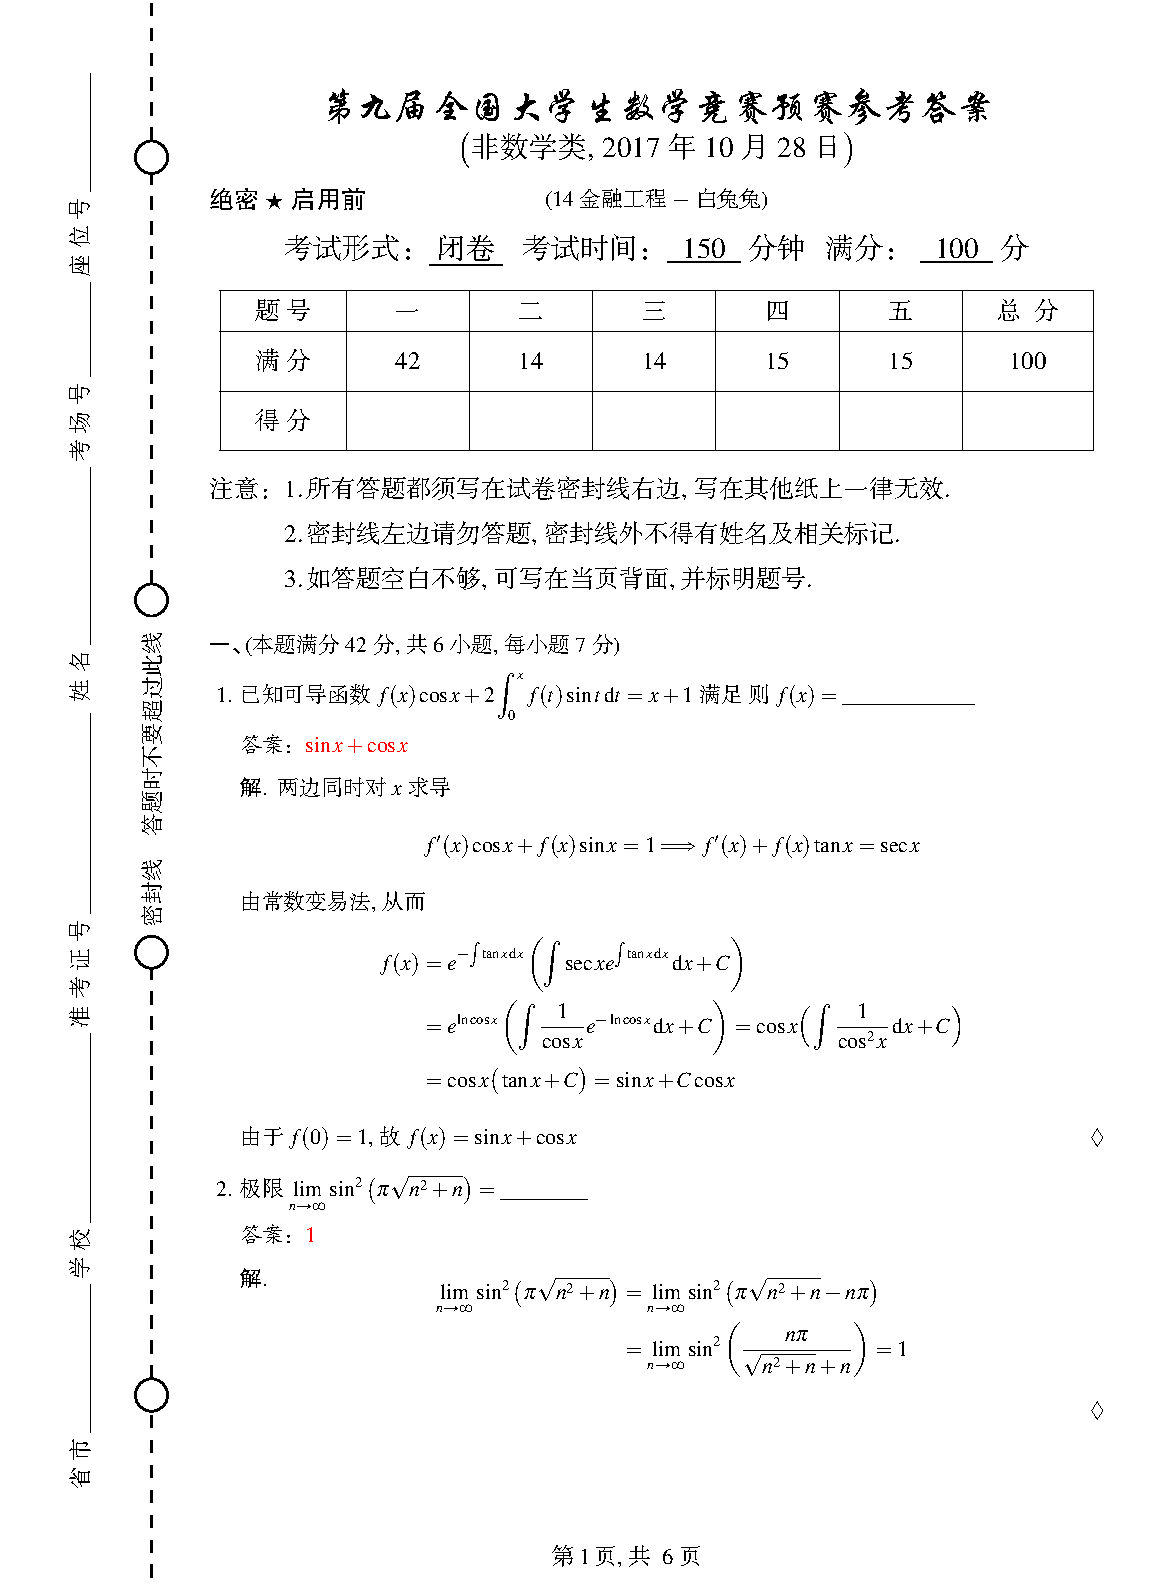
\includepdf[pages=1-6,nup=2x1,scale=1,offset=3mm 0mm,column,delta=-10 -0mm]{17nomathdaan.pdf}	
\end{document}
